\documentclass[a4paper,twoside]{bth}
% BTH THESIS TEMPLATE
%--------------------
% Template version 4.1 -- November 16, 2023
% Update also the Word template. Keep the version numbers in both formats in sync.
%--------------------
% Please change the data below appropriately to fit your thesis.
% The data will be used to generate text in various places on the
% thesis front and inner pages.
%--------------------

% DEGREE NAME. The degree name you are submitting your thesis for.
% This must be one of the following:
% Bachelor programmes:
%    Bachelor of Science in Computer Science
%    Bachelor of Science in Digital Game Development
%    Bachelor of Science in Software Engineering
% Master programmes:
%    Master of Science in Computer Science
%    Master of Science in Software Engineering
%    Master of Science in Telecommunication Systems
% Civilingenjör programmes:
%    Master of Science in Engineering: AI and Machine Learning
%    Master of Science in Engineering: Computer Security
%    Master of Science in Engineering: Game and Software Engineering
%    Master of Science in Engineering: Marine Engineering
%    Master of Science in Engineering: Software Engineering
%    Master of Science in Industrial Management and Engineering
%    Master of Science in Mechanical Engineering
\newcommand{\thesisDegree}{Bachelor of Science in Software Engineering}

% DATE. The month year when your final report was submitted.
\newcommand{\thesisMonth}{May}
\newcommand{\thesisYear}{2024}

% FACULTY.
% Must be either Computing or Engineering.
\newcommand{\faculty}{Engineering}

% COURSE TIME. Course time in weeks.
% For a 15 credits course this should be 10 and
% for a 30 credits course, this should be 20 weeks.
% Note that the week figure is the same whether you work alone or in a pair.
\newcommand{\thesisWeeks}{20}

% TITLE.
\newcommand{\thesisTitle}{Highlights in Counter-strike 2}

% SUBTITLE.
% If you do not have a subtitle, please delete the line below.
\newcommand{\thesisSubtitle}{Creating a new algorithm to find highlights}

% AUTHORS.
% Please replace with your first name(s) and last name(s). There can be several of each.
\newcommand{\authorFirst}{Linus Jansson}
\newcommand{\authorFirstMail}{lijs21@student.bth.se}
% If there is no second author, please delete the texts in the last parentheses.
\newcommand{\authorSecond}{Max Dahlgren}
\newcommand{\authorSecondMail}{mafq21@student.bth.se}

% SUPERVISOR.
% Please replace with title, first and last names of your academic supervisor.
\newcommand{\super}{Dr. Henry Edison}
% Please replace with the name of the department of your academic supervisor, e.g.,
% Computer Science, Mechanical Engineering, etc.
\newcommand{\superAffiliation}{Computer Science}


% PACKAGES AND COMMANDS START
%----------------------------
% please do not delete or change anything before the END of this section
\usepackage{float}
\usepackage[utf8]{inputenc}
\usepackage[T1]{fontenc}
\usepackage{graphicx}
\usepackage{amsmath}
\usepackage{mathenv}
\usepackage{amssymb}
\usepackage{amsthm}
\usepackage{textcomp}
\usepackage{longtable}
\usepackage{multirow}
\usepackage{booktabs}
\usepackage{caption}
\usepackage{pifont}
\usepackage{tikz}
\usepackage{pgfplots}
\usepackage{changepage}
\usepackage{listings}
\usepackage{nameref}
\usepackage{hyperref}
\usepackage{xspace}
\usepackage{xtab}
\usepackage{enumitem}
\usepackage{glossaries}

\graphicspath{{Images/}}

%\usepackage[sort&compress,numbers,square,comma]{natbib} % natbib interferes with the style; use \cite instead (see below)
\usepackage{cite} % works only with numeric citations; comment out when using author-year styles
\usepackage[color=blue!10,textsize=footnotesize,textwidth=25mm]{todonotes}
\DeclareGraphicsExtensions{.pdf}

\newtheorem{lem}{\textsc{Lemma}}[chapter]
\newtheorem{thm}{\textsc{Theorem}}[chapter]
\newtheorem{prop}{\textsc{Proposition}}[chapter]
\newtheorem{post}{Postulate}[chapter]
\newtheorem{corr}{\textsc{Corollary}}[chapter]
\newtheorem{defs}{\textsc{Definition}}[chapter]
\newtheorem{cons}{\textsc{Constraint}}[chapter]
\newtheorem{ex}{\textbf{Example}}[chapter]
\newtheorem{qu}{\textbf{Question}}[chapter]
% -------------------------
% PACKAGES AND COMMANDS END
\makeglossaries
\loadglsentries{glossaries}

\newglossaryentry{latex}
{
    name=latex,
    description={Is a markup language specially suited 
    for scientific documents}
}

% DOCUMENT BEGINS HERE
\begin{document}

\pagestyle{plain}
\pagenumbering{roman}

% THESIS FRONT PAGE (please do not change)
% ----------------------------------------
{\pagestyle{empty}
\changepage{3cm}{1cm}{-0.5cm}{-0.5cm}{}{-1.5cm}{}{}{}
\noindent
\begin{tabular}{@{}p{0.75\textwidth} p{0.25\textwidth}}
\thesisDegree & \hfill\multirow{3}{*}{\bthcsnotextlogo{3cm}} \\
\thesisMonth \ \thesisYear & \\
\end{tabular}

%\begin{center}
\center
\vspace {7.5cm}
{\Huge\textbf{\thesisTitle}}

\vspace {0.5cm}
{\Large\textbf{\thesisSubtitle}}

\vspace{2cm}
{\Large\textbf{\authorFirst}}

\vspace{0.3cm}
{\Large\textbf{\authorSecond}}

\vspace*{\fill}

\noindent\makebox[\linewidth]{\rule{\textwidth}{1pt}} 
Faculty of \faculty, Blekinge Institute of Technology, 371 79 Karlskrona, Sweden
%\end{center}

\clearpage
} % Back to \pagestyle{plain}
% ----------------------------------------


% THESIS INNER PAGE (please do not change)
% ----------------------------------------
{\pagestyle{empty}
\changepage{3cm}{1cm}{-0.5cm}{-0.5cm}{}{-1.5cm}{}{}{}

{\small
\noindent
This thesis is submitted to the Faculty of \faculty\ at Blekinge Institute
of Technology in partial fulfillment of the requirements for the degree of
\thesisDegree. The thesis is equivalent to \thesisWeeks\ weeks of full-time studies.

\vspace{1cm}

\noindent
The authors declare that they are the sole authors of this thesis and that they have
not used any sources other than those listed in the bibliography and identified as references.
They further declare that they have not submitted this thesis at any other institution to
obtain a degree.
}

\vspace{10cm}

\noindent
\textbf{Contact Information:} \\
Author(s): \\
\authorFirst \\
E-mail: \authorFirstMail \\
\\
\authorSecond \\
E-mail: \authorSecondMail

\vspace{2cm}

\noindent
University advisor: \\
\super \\
Department of \superAffiliation

\vspace*{\fill}

\noindent
\begin{tabular}{@{}p{0.5\textwidth} l c l}
Faculty of \faculty              & Internet & : & www.bth.se \\
Blekinge Institute of Technology & Phone    & : & +46 455 38 50 00 \\
SE--371 79 Karlskrona, Sweden    & Fax      & : & +46 455 38 50 57 \\
\end{tabular}
\clearpage
} % Back to \pagestyle{plain}
% ----------------------------------------

\setcounter{page}{1}


%%%%%%%%%%%%%%%%%%%%%%%%
% YOUR TEXTS START HERE
%%%%%%%%%%%%%%%%%%%%%%%%

% ABSTRACT IN ENGLISH
% -------------------
\abstract
\textbf{Our text:}\\
Highlights are often the things people remember from sport events, and are memorable even years after the event has taken place. In the world of e-sport, games such Counter Strike 2 the statement also stands true. We present a new algorithm for creating highlights that takes into account many different metrics to calculate the better moments of a game of Counter Strike 2.
\\\\
\textbf{Their text:}\\
Most readers will turn first to the abstract of your thesis. Use it as an opportunity to spur the reader's interest. The abstract should highlight the main points of your work, especially the thesis' problem statement, methods, findings, and conclusions. However, the abstract does not need to cover every aspect of your work. The main objective is to give the reader a good idea of what the thesis is about.

The abstract should be completed towards the end when you are able to overview your project as a whole. It is nevertheless a good idea to work on a draft continuously. Writing a good abstract can be difficult since it should only include the most important points of your work. But this is also why working on your abstract can be so useful -- it forces you to identify the key elements of your degree project.

Structured abstracts have several advantages for authors and readers. They help readers to quickly find information in an abstract and also guide authors in summarizing the content of their manuscripts precisely. Below you find the main components of a structured abstract.

\noindent
\textbf{Background.} ... \newline
\textbf{Objectives.} ... \newline
\textbf{Methods.} ... \newline
\textbf{Results.} ... \newline
\textbf{Conclusions.} ...

\vspace{1cm}
% You can list up to 5 keywords, at most 2 appearing in the title;
% starts 1 line below the abstract.
\noindent
\textbf{Keywords:} Up to 5 keywords, at most 2 of these should appear in the title. Starts 1 line below the abstract.

\cleardoublepage
% -------------------




% ACKNOWLEDGEMENTS
% -------------------
\acknowledgments % Optional, comment out this part if not needed
\noindent
Here you can add your acknowledgements.

\cleardoublepage
% -------------------


% TABLE OF CONTENTS PAGES (generated by LaTeX using the command(s) below)
\setcounter{secnumdepth}{3} % only include sections down to level 3
\tableofcontents
% You should uncomment the commands you need.
\listoffigures             % in case you have them
%\listoftables              % in case you have them
%\listofalgorithms          % in case you have them

\cleardoublepage
\pagestyle{headings}
\pagenumbering{arabic}
\printglossaries
\gls{latex}.


%------------------------------
% THE ACTUAL THESIS STARTS HERE
% The chapters below are just suggestions and need to be adapted to your topic.

\chapter{Introduction}
\label{chp:introduction}  % labels are used for cross references
\section{On the content}
Your introduction has two main purposes: 1) to give an overview of the main points of your thesis, and 2) to awaken the reader's interest. It is recommended to rewrite the introduction one last time when all writing is done, to ensure that it connects well with your conclusion.

\emph{Tip}: For a nice, stylistic twist to create a connection between your introduction and your conclusion you can reuse a theme from the introduction in your conclusion. For example, you might present a particular scenario in one way in your introduction, and then return to it in your conclusion from a different -- richer or contrasting -- perspective.

The introduction should include:
\begin{itemize}
    \item The background for your choice of theme
    \item A problem statement that defines the scope of your thesis
    \item A schematic outline of the remainder of your thesis 
\end{itemize}


\section{Background}
\textbf{Our text:}\\
In Counter Strike there are two teams, the Terrorists (T) and Counter-terrorists (CT). The game is focused on the T side planting a bomb at one of two sites, and the CT defending that site and defusing the bomb. This game is highly mechanical, meaning that its skill ceiling is very high. Each game in Counter Strike 2 is play with first to 13, with 12 round halves. There is overtime if the score is even after 24 rounds. Overtime consists of 3 rounds per side, with the first to win four rounds winning the game.
\\\\
All tournaments have different group stages, but most if not all use the single elimination bracket for the playoffs. Meaning there is a quarter, semi and final rounds, often best of 3 wins in the quarter and semi-finals and best of 5 in the finals.
\\\\
Millions of players tune in to watch professional matches, with the highest peak viewers up close to 3 million(2.75) people watching. This game was the PGL major in Stockholm, during the finals, when G2 faced NaVi, and the game was very close, going all the way to game 5.
\\\\
In the world of Counter Strike, there are a few moments that all players of the game are familiar with. These are often plays that work against all odds, with everything at stake. A few of these moments are when the players such as S1mple, during ESL One New York 2016, throws his AWP, the best gun in the game to confuse his opponent on dust\_2, or the one where Twistzz just pushing through the defense on the map Nuke during IEM Cologne 2022, or, probably the most iconic of all, Coldzeras B site hold on the map mirage, at MLG Columbus 2016. He single handily stopped Team Liquid from winning the game, with the score at 15-9 for Liquid. This, combined with the skill and luck involved, makes this probably the most recognized Counter Strike highlight of all time.\\\\
Team liquid is approaching bomb site B with all of its members through what is called apartments. Coldzera is holding this part of the map scooped in with his AWP. The first player leading the push gets spotted by Coldzeras and gets eliminated. The four remaining members of Team liquid starts pushing toward Coldzera as he repositions to a new spot. Coldzera then does the most unthinkable play in his position and jump fires without scoping his AWP significantly decreasing the accuracy of the gun. He eliminates two opponents with this risky play and with only two opponents left he finishes off the fourth opponent with a quick no-scope and his teammate TACO eliminates the last standing member of team liquid. \\\\
They go on to win that major, many thanks to this play. Highlights like this are what most people watch competitive e-sports for, and if you watch the highlight, you can hear how the crowd loves the play, and the casters are impressed.\\\\
Most players playing Counter Strike, have these moments themselves, perhaps with less on the line, but the feeling of holding down a part of the map by yourself, is a great feeling. Some people compile all of their best moments into a highlight reel to upload for people to see. Our question is, can we find these highlights by analyzing the game, and find better highlights for a given round, in a given game from a given player. We are going to research if that is possible, how that could be done, and if getting highlights from your own matches, improves enjoyment of the game.\\\\
A highlight is when something extraordinary occurs during a time period or an event. In the case of Counter-Strike 2 a highlight could be a multitude of things, for example a round when a player kills multiple players in one round or a player kills more than one player with one bullet or a single utility.\\\\
A lot of things occur during a Counter-Strike 2 match, meaning it can be hard to decide what highlight is better than another. In a single game, multiple highlight worthy moments might happen, such as in one round a player might eliminate the whole enemy team, while in another round a player might kill three players with one grenade. It is here the algorithm comes in and values each play with different metrics and can decide which round would be better to make a highlight out of.\\\\


\section{Defining the scope of your thesis}
\textbf{Our text:}\\
This thesis will focus on the creation of our new algorithm and the empirical research we have conducted to create a better algorithm for finding highlights in the video game Counter Strike 2. The thesis will also research if there is a noticeable difference between what a novice player and seasoned player of the game prefers in a highlight.
\\\\

\chapter{Related Work}
\label{chp:relatedwork}
\section{On the content}
\textbf{our text:}\\
In the article \cite{Tgwri1s2017} by Tgwrils (2017) we can further research into how the new rating system works and this gives us a better insight of how we can rate our metrics for the algorithm. The rating system is explained in the article as rating performance and not rating individual highlight moments. It focuses more on the overall performance of a player over a match. 
\\\\
In the paper \cite{Rubin2022} by Rubin, A. (2022, January 13). There are a lot of useful metrics and data we can use, such as what is the most significant factor for a team to win a round, Rubin presents data that show that the team's equipment value is one of the leading causes for a chance to win. This information we can take into account when creating our new algorithm. We can for example interpret this as if a player with poorer equipment value eliminates the enemy team, it is higher valued in the algorithm than if the player had more valuable equipment.\\\\ 
It is also stated how they analyze data from games and parse the demos they collected, which is of great use to us as we also need to collect similar data.\\\\
In the article "On broadcasted game video analysis: event detection, highlight detection, and highlight forecast" by Chu, W.-T. and Chou, Y.-C. (2016) they go over the topic of highlight detection which is appropriate for us. They go over metrics such as motion intensity, frame dynamics, number of gamers, event ratio, number of viewers chat and number of emotion symbols. All of these metrics might not be possible to collect as we are not analyzing a live event where there are any active viewers or interaction with any chat or crowd. As the article does however cover the topic of arousal of viewers, it is worth studying as the purpose of a highlight is to create excitement.\\\\
In the paper  "Automatic soccer video analysis and summarization," by m A. Ekin, A. M. Tekalp and R. Mehrotra (2003). We get to read on how a very different sport handles video analysis and summarization of games. The text is interested in the sense how other sports/activities can be analyzed and what to can be looked at, for example in the article there is mentioning of slow-motion segments which could also be used in highlights to show the event in more detail.
\\\\
In the master thesis "CS:GO Player Skill Prediction" \cite{BaranNama} we get to read about 
\\\\
The articles mentioned covers different aspects of analyzing games via metrics, this relates to our work as to find highlights we need to analyze the game similarly. 

\chapter{Method (HOW)}
\label{chp:method}
\section{On the content}
Here you specify and motivate your research questions or hypotheses and relate them to your overall goal, research question, or hypothesis, if you have defined one in the introduction. Furthermore, you describe the method or research design for answering your research questions or testing your hypotheses and discuss the reliability and validity of your approach. The latter is important for a reader to assess the trustworthiness and generalizability of your results.  


\section{Defining research questions}

\section{Preliminary goals:}
\normalsize
\begin{enumerate}[label=PG\arabic*., leftmargin=*]
    \item Create a proof of concept of a highlight algorithm, that finds "better" highlights for a given player in a match
    \item Find out what is required for an alternative highlight algorithm, what metrics players prefer
    \item Find what makes a highlight "better" and increases enjoyment when watching a highlight.
\end{enumerate}

\section{Preliminary research questions:}
\normalsize
\begin{enumerate}[label=RQ\arabic*., leftmargin=*]
    \item How can one create an algorithm to find better highlights in Counter Strike 2? \\\\
    The value of creating the proof of concept is a better highlighting algorithm than existing ones, thus making for better clips for players and spectators of the game. 
    \item What metrics are most important when developing an algorithm to find highlights in Counter-Strike 2? \\\\
    Finding out what is required for a highlight and what players prefer can help in further research into the subject and can even connect to other games where similar highlights can be of interest.
    \item How do the perceptions of what makes a good highlight differ between novice and experienced players?\\\\
    Finding out the difference between perception of highlights of a seasoned player or someone who has not as much or no experience gives us a insight how you can direct highlights so that they can be enjoyed by different demographics. 
    
\end{enumerate}
Research question number 1 is connected to goal 1. Question 2 is connected to goal 2. Question 3 is connected to goal 3.\\\\
The value of these goals can affect and be used by players of the Counter Strike 2, others that are interested in the topic of highlight making/analyzing, and for spectators of the game.\\\\

\section{Describing your research method}
We use a proof of concept and mixed-methods approach with surveys and interviews in this study. The interviews are conducted to get a better insight into what and how to weigh different metrics that will be used in the algorithm. The surveys serve the purpose of comparing our algorithm with existing highlight tools. This way we can see if our algorithm could be considered better at finding highlights.
\subsection{Proof of concept of an algorithm}

\subsubsection{Initial plan}
The initial plan was to have a system in which the \Gls{Demofile} is analyzed and all the results of the different metrics are multiplied by a weight and then added to a final score. Some of the metrics are ones that you want to be lower, like the time between each kill, and if you die. The formula would look something like this.

$$\text{Total Score} = \sum_{i=0}^{x} weight_i \times metric_i $$

where x is the number of metrics

\subsubsection{Implementation}

Implementing the analyzer step was a lot of code to write, but not much advanced code. Mostly it was reading some value for each player every round, and storing those values in a Metrics class. This class held all information about a players metric for a given round, and contained some helper methods to set the metrics in a cleaner way.

One of the metrics that was hard to implement was the \Gls{jumpshot}s. Until very recently (2024-04-24), there was no built in way of checking if a player was in the air or not, but right in time, Valve, the developer of Counter strike 2, added a new feature\cite{onTheOtherHandReleaseNotes} to show if a player is in the air during a kill.

Before this, our solution was to check the Y position of the player over a two second windows, one second before until one second after. After this, we checked the position of the player and made sure that the players velocity was an arch, starting going high, and then curving back down. This solution has issues, a ladder or stairs could fool this solution, so the newer update was very helpful.

\subsubsection{Final Product}

The final product contains a web interface, that made it easier for us to use and look at the metrics and whats going on. This was helpful for debugging issues with the analyzer, as well to see why a round got the score it did. The full process is that you upload the demo file you want to analyze onto the site, this gets passed to a DemoAnalyzer instance, that extracts the demo information. This then loads up a page where we can see all the metrics, for all the players, in all rounds. The round score for each round is automatically calculated, and the best round score of the match gets displayed on the site, along with the metrics for that round. This is how we determined what clips were supposed to be used for the survey. The web page could be adapted for user consumption, by just hiding the details of the round.

\paragraph{Linear Metrics}
For all linear metrics that we have, we map the input to somewhere between 0 - 100. This was we handle cases where two metrics are of the same importance, but the value they give are orders of magnitude off each other. An example would be damage, and kills (genom) smokes. You can only get a maximum of 5 kills trough smokes, but you can get up to 500 damage. This was if i get 2 smoke kills and 200 damage, both will output 40. We used a linear mapping function for this. The function is explained below

The metrics that use this method of scoring is:
\begin{itemize}
    \item Damage dealt
    \item Head shots
    \item No-Scopes
    \item How long between each kill
    \item \Gls{jumpshot}s
    \item Hit ratio
    \item Distance
\end{itemize}

\begin{align*}
& \textbf{Function map:} \\
& \text{map}(v, v_{\text{min}}, v_{\text{max}}, t_{\text{min}}, t_{\text{max}}) = \frac{v - v_{\text{min}}}{v_{\text{max}} - v_{\text{min}}} \cdot (t_{\text{max}} - t_{\text{min}}) + t_{\text{min}} \\
& \quad \text{where:}\\
& \quad \quad v: \text{input value}\\
& \quad \quad v_{\text{min}}: \text{minimum input value}\\
& \quad \quad v_{\text{max}}: \text{maximum input value}\\
& \quad \quad t_{\text{min}}: \text{minimum target value}\\
& \quad \quad t_{\text{max}}: \text{maximum target value}\\ \\
& \textbf{Function mapToScore:} \\
& \text{mapToScore}(v, v_{\text{min}}, v_{\text{max}}) = \text{map}(v, v_{\text{min}}, v_{\text{max}}, 0, P) \\
& \quad \text{where:}\\
& \quad \quad P:  \text{represents the constant POINTS\_PER\_METRIC = 100}
\end{align*}

This function is the same used by a popular library p5js \cite{p5jsMap}, that is used for interactive graphics among other things. We made a shorthand to write cleaner code, using the function mapToScore, that calls the map function, but with the target min and max values already set to 0 and POINTS\_PER\_METRIC, that in out case is 100


\paragraph{Exponential metric}
For some metrics, we choose to make a greater difference between the lower numbers and the higher ones. We did this by raising the input to the power of 2 before using the mapToScore function. This was we get a bigger difference between 4 and 5, compared to 2,3. This we only did for kills.

\paragraph{Other metrics}
Some metrics did not work well with this system, since they either are not numbers, or needed other processing on them to make them work well inside the algorithm. This section will explain how they work, and why they did not work with the linear or exponential functions. Some of them just mapped to either the maximum amount of points, like if you died, or what side you were on.
\paragraph{HP left}

This uses a exponential decay function. This is because the lower the health of the player, the more stress it puts on the player. \todo{reference to interviews, and write more about why we choose 35}. We picked 35 as the point where we should start increasing the points significantly. We can now input the \acrshort{hp} of the player into the formula and we get a value between 5 and 100.            
$$x) = 100 \cdot e^{-ax}  \qquad \text{where } a = 0.03$$
This is then mapped using the function mapToScore from before to a number between 0 and 100. After the normalizing we multiply this by the weight for the metric. 
\todo{explain how the function works and how we came p with it}
This formula is an exponential decay function. It models the decrease in \acrshort{hp} Left Value as the input value (x) increases. The growth rate (a) controls how quickly the value decays. A higher growth rate means a faster decay. \todo{CHATGPT WRITTEN}

We choose 0.03 as the $a$ value since this makes the points for that metric go up around the 35 \acrshort{hp} mark, that being one shot away from death from most strong weapons.


\begin{figure}
    \centering
    \begin{tikzpicture}
\begin{axis}[
    axis lines = left,
    xlabel = $HP$,
    ylabel = {$f(x)$},
]
\addplot [
    domain=0:100, 
    samples=100, 
    color=blue,
] {100 * exp(-0.03*x)};
\addplot[
    only marks,
    mark=*,
    nodes near coords,
    point meta=explicit symbolic,
]
coordinates {
    (35, 100 * exp(-0.03*35)) [One Shot]
};
\end{axis}
\end{tikzpicture}
    \caption{HP left scaling}
    \label{fig:hp-left}
\end{figure}

\paragraph{Weapon score}
For the weapons, we decided to score each weapon individually, this was each weapon gets a part of the max score for the metric. This is done by first dividing the total score for the metric, so for four weapons that will be 25 points. Then it used that value as the max points for the weapon, and rates it with the difficulty rating from the game, taken from the ingame buy menu. For an ak47, which has a difficulty rating of 4, the formula is as follows: $$ score = map(weaponDifficulty, 0, MWW, 0, PPW) $$ Here MWW is max weapon weight, and PPW is points per weapon.

This is done for each one of the weapons added together and finally multiplied with the weight for guns.


\paragraph{Side}
When looking at what side the player is playing on, either \acrshort{t} or \acrshort{ct}, we looked at the win rate for each side for the last 6 months\cite{hltvMapStats}. Here we saw a quite even split, but based on the map in the current competitive map pool, \acrshort{ct} has a higher win rate on the majority of the maps. Therefore we assign \acrshort{t} and \acrshort{ct} -1 and 1, then in the weights, it has a negative value, so that the -1 for \acrshort{t} get awarded more points than \acrshort{ct}.


\subsubsection{Technologies used}
Our algorithm was built using Typescript as the language of choice. This choice was made both out of familiarity and based on Typescripts fast iteration speed, enabling us to make changes faster than a language like C++ or Rust.

Counter-strike 2 records everything that happens in a match in a \Gls{demo} file. To parse this information, we used a library\cite{demoparser} that would give us events from the match, such as whenever a player dies, shoots, or when the rounds start or end. This library does not give us the data we need directly, so for that we need to parse information from the events available. So for that we need to analyze the data from the demo, to later pass to our algorithm to calculate with \todo{EXPLAIN MORE????}
\subsubsection{How it works}
The first part of the process to generate a highlight is to extract the metrics from the demo file. This is done in a file called DemoAnalyzer.ts, and this fine handles reading the \Gls{demo} file and transforming the data into a usable format. It does this by looking at different events \todo{list events??} and calculate the metrics. \todo{explain how some of them work?}.

The next part is to store the metrics in the database. This is handled by a separate file `SaveDemoInfo.ts`. This file reads the data, and puts it into tables in the database. The reason for making this a separate step was for readability and code quality. This splits up the code into the analyzer, that is only responsible for reading the data, and storing it in memory, and the SaveDemoInfo part, that only focuses on storing the data. 

The last part is the most important step. This is the algorithm itself. This takes in all the data from the demo file, as well as the weights we have defined from the interviews \ref{sec:interviews}. This then calculates a score from each metric between 0 and 100. This was done to make sure that each metric is valued the same before the weighing process. This is done using this mapping function from p5.js\cite{p5jsMap}\todo{check ref with henry}

After the mapping function has given its value between 0 and 100, this then is weighted, so that we can control how important the metrics are for a highlight. For example, should one kill through a wall be considered better or worse than one kill that is very far away? That is the proposal of a weight. \todo{better example?}

\subsection{Survey}
\label{sec:survey}
A survey will be created with our algorithm's outputted round and the Allstar{glossarie} tool's "play of the game" round, where the same matches are evaluated on the same player, and the participant can choose which they prefer. Both rounds will be re-recorded so that a fair comparison can be made without editing and each clip starts a few seconds before and action such as shooting, spotting an enemy or throwing utility is done.\\\\
\textbf {Content for the survey:}
\begin{itemize}
    \item The respondent will be prompted to answer a question about how familiar they are with the game Counter-Strike 2. This will be presented in a type of likert scale. 
    \begin{figure}[H]
        \centering
        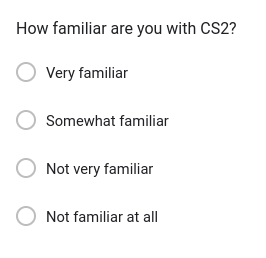
\includegraphics[width=4cm]{Images/likertscale.png}
        \caption{Likert scale}
        \label{fig:likerScale}
    \end{figure}
    \item Two clips are shown, A and B. One is the round our algorithm picked and one is the round Allstar picked, the respondent will not be told which clip is which so that there will be no biases. The respondent is then faced with the question of which clip they preferred or if the clips are indifferent. They then have the choice to write a more detailed explanation why they picked as they did or any other input they had. There will be 18 clips in total, 9 comparisons.
    \begin{figure}[H]
        \centering
        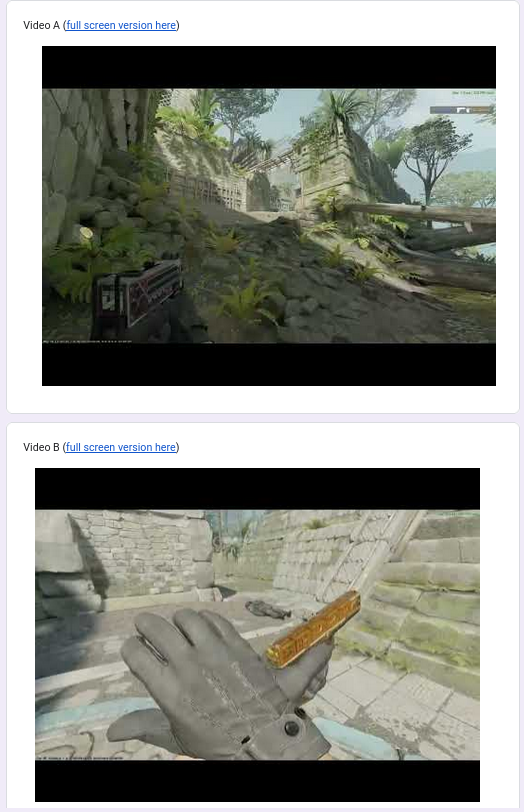
\includegraphics[width=10cm]{Images/A-B_choices.png}
        \caption{Video A and B example}
        \label{fig:VideoA_B}
    \end{figure}
    \begin{figure}[H]
        \centering
        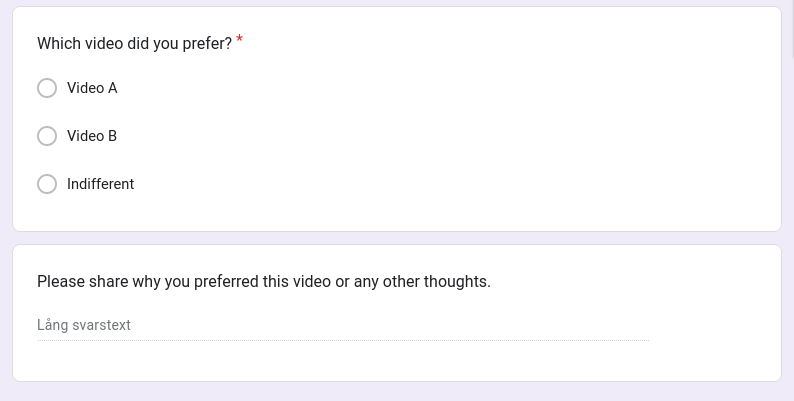
\includegraphics[width=10cm]{Images/Questions_AB_reason_Survey.png}
        \caption{Video A and B example}
        \label{fig:VideoA_B_answer_reason}
    \end{figure}

\end{itemize}
The survey will connect with preliminary goal 1 to see if our the highlight our algorithm creates are preferred over what existing tools create. It will also answer research question 3 by seeing if algorithm based highlight clips can create joy for the viewer.\\\\
The choice to conduct surveys was made because we want to have a large pool of opinions, as we want to see if our new algorithm is "better" than existing ones. By choosing to do surveys, we can reach a greater amount of people. To create the surveys, we would use either sites like Surveymonkey.com or Google Forms. The surveys would be put in different forums on sites like Reddit.com, Discord channels and HLTV.org. The main targeted respondents would be those who have played Counter Strike 2, as these are the more likely to have an opinion about the clips they are shown. As we have no control of the surveys and who receives them, we would likely need to put questions such as "Have you played the game Counter Strike 2?" to see the difference in opinions between people who have played the game and not.\\\\
When analyzing the results, we would need to do a statistical analysis of the quantitative data, which would be the preferred clip. We could then gather statics such as the median for which clips the users decide to pick. Creating pie charts would also be a good way to visualize how the participants picked. For the qualitative data, which would be the free text part where the participant explained why they picked what, we will have to look for patterns and trends between what they picked and categorize based on if they played the game before.

\subsection{Interviews}
\label{sec:interviews}
Interviews will be conducted before developing the algorithm to find what metrics players weigh higher, to give a better baseline on what the weights should be. \\ \\
\textbf {Questions for the pre interview:}\\
\section{Questions:}
\normalsize
\begin{itemize}
    \item What is the most memorable highlight in Counter Strike history according to you? 
    \begin{itemize}
        \item What makes it memorable?
    \end{itemize}
    \item What is your experience with highlights in FPS games?
    \item What makes a good highlight?
    \item What metrics are important for a highlight?
    \item Rate these metrics from 1 to 10:
        \begin{itemize}
        \item Amount of kills 
        \item if the player died
        \item Weapon used 
        \item Time between each kill
        \item Bullets fired
        \item Team side
        \item Player position (Distance)
        \item Airborne 
        \item Headshot
        \item Damage given
        \item HP of the player
        \item No scope with scoped weapons
        \item Wall banging
    \end{itemize}
    \item Do you use any highlight tool?
    \begin{itemize}
        \item What highlight tool?
        \item What do you do with the highlights?
    \end{itemize}

    
\end{itemize}

Question one to three in the pre interview will help us achieve the three preliminary goals and answer the research questions, as these will give us further insight into what metrics are needed and how to value them. It will also help us get a better insight to what makes a good highlight. \\\\
The choice of doing interviews was so that we could get a better understanding on how to rate different metrics and what players think is a good highlight so that we could improve our algorithm. The interview would be conducted either in person or online, where it would be recorded or transcribed. The targeted respondents would be people who analyze the game, such as casters, commentators or professionals players of the game. We would also interview more casual players of the game. To recruit these respondents, we would have to email or contact them through other forms and ask if they are interested in participating in our interview. After the interviews are conducted, we gather all the data we have collected and analyze it. Things to look for would be patterns and themes that are recurring in the answers.\\\\
The answers we gathered here lays a base on how we weigh our metrics but could be used in other games that are similar to Counter Strike 2.\\\\ 

\section{Validity and reliability of your approach}
Our approaches of collecting data through interviews was done via discord where we recorded the interview. This was done so that we could have a greater reach of who we interviewed. This made it possible to get a bigger size pool of different people. We also had to take into account that the people we wanted to interview had played Counter Strike or similar games.\\\\ We recognized that it would be hard to fairly value metrics, as there a many, but the approach we took made it so that if there are metrics not mentioned by us in the interview the interviewee could have the possibility to add metrics.\\\\
Our approaches of collecting data through surveys was done via Google forms to compare our algorithm with the existing highlight tool ALLSTAR. The participants would not know which clip came from ALLSTAR or our algorithm. As the clips created are from the same matches and the same persons when comparing this makes it as un-biased as possible. The games where from our own games history from the dates {INSERT DATE} to {INSERT DATE}. In case our algorithm and Allstar outputted the same round a new match was picked and the instance noted down. 
\chapter{Results and Analysis WHAT}
\label{chp:results}
\section{On the content}
\section{Survey results}
\label{chp:surveyResults}
Looking at the survey results, we can see that our algorithm won $\frac{2}{3}$ of the times, as can be seen in figure \ref{fig:surveyOverall}. This indicates that our algorithm is more suitable for finding highlights for certain types of players. Most of the respondents were very familiar with the game, showing that experienced players seemed to like our implementation.
\begin{figure}
\centering
\begin{tikzpicture}[object/.style={thin,double,<->}]
 \pie{66.6/Our algorithm,33.3/Allstar} 
\end{tikzpicture}
\caption{Pie chart showing what algorithm won in the survey}
\label{fig:surveyOverall}
\end{figure}
\subsection{Match 1}
\textbf{old text}
In the first match, our algorithm just took the win. It is not a large win by any stretch of the imagination, but based on the comments added by the respondent, both highlights are very close. However, a respondent said that Video A was more tactical, but that both clips were clean. Another user, who preferred Video B, said that that play was more fearless. The people that choose B seemed to think video B has more action and better decision making. The people who chose A commented on how \gls{clean} it was

For this set of highlights, video A won by a slim margin. The people that taught video a was the better one commented on that it was more tactical and \gls{clean}. That the AK47 was used instead of the glock also attracted some viewers. One respondent said that; "It was a good clutch". The respondents that liked video B had the opinion that that highlight had more action. The people who responded indifferently mentioned that both clips were the same in terms of level of game play.

\textbf{URLS HERE}
\begin{figure}
\centering
\begin{tikzpicture}[object/.style={thin,double,<->}]
 \pie{40/ Video A (Our algorithm),36/Video B (AllStar), 24/Indifferent} 
\end{tikzpicture}
\caption{Result from Match 1}
\label{fig:match1}
\end{figure}


\subsection{Match 2}
For this set of highlights, video B took the win, with a little more than half of the respondents liking this highlight more. Respondents mentioned that the knife kill during video B was a large factor, and that the kills were all solo plays, with no help from teammates. They also mentioned that video A was more messy and video B was more clean.


\textbf{URLS HERE}
\begin{figure}
\centering
\begin{tikzpicture}[object/.style={thin,double,<->}]
 \pie{34.6/ Video A (Our algorithm),57.7/Video B (AllStar), 7.7/Indifferent} 
\end{tikzpicture}
\caption{Result from Match 2}
\label{fig:match2}
\end{figure}
\subsection{Match 3}
For this set of highlights Video B was the winning highlight. While several viewers liked the impressive 4K spraydown and first kills in Video A, the majority found the gameplay in Video B to be better.

Some comments highlighted specific reasons why Video B was more appealing.

\begin{itemize}
\item \textbf{Better decision-making:} One respondent said that "The Read on The Game is on the 2nd Video way more accurate."
\item \textbf{Map awareness:} Another respondent said "Better checks on corners."
\item \textbf{Overall gameplay:} Several viewers simply stated their preference for Video B, indicating a more enjoyable viewing experience.
\end{itemize}

\textbf{URLS HERE}
\begin{figure}
\centering
\begin{tikzpicture}[object/.style={thin,double,<->}]
 \pie{65.4/ Video B (Our algorithm),19.2/Video A (AllStar), 15.4/Indifferent} 
\end{tikzpicture}
\caption{Result from Match 3}
\label{fig:match3}
\end{figure}
\subsection{Match 4}


For this set of highlights Video B was the winning highlight for a few reasons.

\begin{itemize}
\item \textbf{Fast-paced action:} One respondent stated, "Video B was way fast paced, which I like more."
\item \textbf{Strategic gameplay:} One respondent commented: "Just a better round, he knows what he is doing and plays around the enemies making mistakes" which shows a more calculated approach to the game.
\item \textbf{Map control:} Another viewer noted that "Video B felt like it opened up an A push pretty cleanly," showing that taking initiative, and opening up a site makes a good highlight.
\end{itemize}

Overall, viewers found Video B to be a better highlight, due to its faster and more strategic gameplay. The criticism of Video A mentioned a hesitation to push forward, and some bad mechanics regarding jump spotting.
\textbf{URLS HERE}
\begin{figure}
\centering
\begin{tikzpicture}[object/.style={thin,double,<->}]
 \pie{50/ Video B (Our algorithm),42.3/Video A (AllStar), 7.7/Indifferent} 
\end{tikzpicture}
\caption{Result from Match 4}
\label{fig:match4}
\end{figure}
\subsection{Match 5}


People liked Video B more in this set of highlights.
The reasons that the respondents liked video B more:

\begin{itemize}
\item \textbf{Used smoke well:} "Played the smoke (very nice!) on video B"
\item \textbf{Got more kills:} "In video B he does not die, and gets most of the kills"
\item \textbf{Won the round:} "He didnt die, and won round"
\end{itemize}

While some people liked the skills shown in Video A, most preferred Video B because the player made good choices and won their team the round, as well as he did not die.
\textbf{URLS HERE}
\begin{figure}
\centering
\begin{tikzpicture}[object/.style={thin,double,<->}]
 \pie{57.7/ Video B (Our algorithm),34.6/Video A (AllStar), 7.7/Indifferent} 
\end{tikzpicture}
\caption{Result from Match 5}
\label{fig:match5}
\end{figure}
\subsection{Match 6}

Most people liked Video B more, saying it had cleaner kills. Some people liked Video A because it was fast-paced and showed teamwork.

The difference between the highlights were:
\begin{itemize}
\item \textbf{Video A - Fast and teamwork:} Some respondents liked how Video A was quicker and showed the whole team working together.
\item \textbf{Video B - Cleaner kills:} Others thought the kills in Video B looked nicer and smoother.
\end{itemize}

A few respondents said both videos were good and bad in different ways. Some also mentioned the teamkills during that round.

\textbf{URLS HERE}
\begin{figure}
\centering
\begin{tikzpicture}[object/.style={thin,double,<->}]
 \pie{38.5/ Video A (Our algorithm),46.2/Video B (AllStar), 15.4/Indifferent} 
\end{tikzpicture}
\caption{Result from Match 6}
\label{fig:match6}
\end{figure}
\subsection{Match 7}
The survey results shows that people liked Video A more. Video A had more kills, including a cool 2-kill spraydown, and the player got the last kill. Some people also liked that it was faster-paced.

\begin{itemize}
\item \textbf{More kills and a cool spray:} "More kills, aswell as a nice 2K spraydown."
\item \textbf{Got the last kill:} "He made the last kill himself in Video A liked that better."
\item \textbf{Faster pace:} "it was also way more fast paced."
\end{itemize}

Some people liked Video B and thought the player made smarter choices, but overall, Video A was more popular.
\textbf{URLS HERE}
\begin{figure}
\centering
\begin{tikzpicture}[object/.style={thin,double,<->}]
 \pie{46.2/ Video B (Our algorithm),38.5/Video A (AllStar), 15.4/Indifferent} 
\end{tikzpicture}
\caption{Result from Match 7}
\label{fig:match7}
\end{figure}
\subsection{Match 8}
The survey shows that video A was the preferred highlight, particularly for the clutch situation, cleaner kills, and higher kill count. While Video B was liked for its efficient 3K, some respondents noted the opponent's missed AWP shots as a huge reason that the highlight even was possible.

\begin{itemize}
\item \textbf{Video A's clutch and kills:} Several viewers favored Video A for the player's ability to secure kills in a clutch situation and the overall higher kill count.
\item \textbf{Video A's cleaner kills:} Some viewers specifically mentioned that the kills in Video A were cleaner and more impressive.
\item \textbf{Video B's methodical 3K:} While acknowledging the skill involved in the 3K in Video B, viewers also pointed out the opponent's missed AWP shots was the only reason this highlight was possible.
\end{itemize}

Overall, the respondents liked Video A for its clutch, and higher kill count and overall was cleaner and Video B was liked for its systematic approach even tho some luck was involved.
\textbf{URLS HERE}
\begin{figure}
\centering
\begin{tikzpicture}[object/.style={thin,double,<->}]
 \pie{65.4/ Video A (Our algorithm),26.9/Video B (AllStar), 7.7/Indifferent} 
\end{tikzpicture}
\caption{Result from Match 8}
\label{fig:match8}
\end{figure}
\subsection{Match 9}

Video B won here due to its better game sense, and that it was fast-paced. The highlight was long and showed that it took a long time for the player to win the round.
The reasoning given from the respondents were:

\begin{itemize}
\item \textbf{Video B's better kills:} Multiple viewers highlighted Video B's better kills, with one specifically mentioning the "clean glock 2K."
\item \textbf{Fast-paced action:} Viewers enjoyed the fast pace of Video B, particularly the initial kills.
\end{itemize}
\textbf{URLS HERE}
\begin{figure}
\centering
\begin{tikzpicture}[object/.style={thin,double,<->}]
 \pie{26.9/ Video A (Our algorithm),61.5/Video B (AllStar), 11.5/Indifferent} 
\end{tikzpicture}
\caption{Result from Match 9}
\label{fig:match9}
\end{figure}

\section{How can one create an algorithm to find better highlights in Counter Strike 2}
The first thing one needs to do is to figure out what metrics should be included in the algorithm. Here, you could interview people in the scene with experience, like casters, analysts, and players of the game. You can also study popular highlights from the community, and see what metrics are the highest in the highlights you watched, and use that as a baseline for what metrics are important to include in highlights. 

Next step in the process to create an algorithm for highlights is to extract the data. Here there is a few approaches that you can take. There is the approach that we took, which is implementing a parser step, to extract all relevant data from the demo file, and gives it into an workable format for the algorithm. Another way to do this is to analyze the video feed from either a screen capture or from a video file. This would require looking at properties of the video / stream, for example watching the kill feed or chat with OCR, and extract data from that, as well as other game information from the UI. Another approach is to use Counter Strike game state integration to get the data in real time from the game itself during the match. This would allow taking a clip of the user screen instead of having to render the clip on a separate server. The game state integration provides much the same data as a demo file would, but in real time.

Once the data has been collected, you would need to analyze that somehow. This is the most "free" part. Depending on what you want to include in the highlights, this will differ a lot. In our case, we focused on mechanical plays, like kills and the skill of the player, but another way would be to focus on funny plays.

Once this is done, the last part is to output the round number of the highlight, and what player did the highlight. Processing this and rendering the highlight is outside the scope of this algorithm.
\section{What metrics are most important when developing an algorithm to find highlights in Counter Strike 2}
To find what metrics, that are important for Counter Strike 2 highlights, we conducted interviews. In these interviews, we got different results:
\paragraph{What is your experience with Counter-Strike or other FPS games?}
2 out of the 7 had little to no experience with the game Counter Strike, but 6 out of 7 had played similar games.
\paragraph{What is your experience with highlights in FPS games?}
2 out of the 7 interviewees had no experience with highlights from FPS games.\\\\
\paragraph{What do you think is the most memorable highlight in Counter Strike history?}
6 out the 7 interviewees answered this question:
\begin{itemize}
    \item "I think the happy 1Deag ace on Banana" (Participant B1, personal communication, April 21, 2024)
    \item "Yes absolutely. After all, I have both famous ones from big tournaments or matches like Coldzera when he jumps and shoots on Mirage."(Participant L1, personal communication, April 10, 2024)
    \item "When you get a four K. It's cool stuff like that." (Participant O1, personal communication, April 30, 2024)
    \item "I think that when you kill a whole team, that's like you just rampage." (Participant O2, personal communication, April 16, 2024)
    \item "But if I'm off the cuff, what pops into my head is Hiko. When he was clutching Dust 2 or something like that."(Participant A1, personal communication, April 09, 2024)
    \item "It's probably OlofPass actually. Because then I was there when he made that boost."(Participant J1, personal communication, April 26, 2024)
\end{itemize}
\paragraph{What makes it memorable?}
Those who mentioned a specific clip said:
\begin{itemize}
    \item "The casters. Caster. Yeah. I suppose also the importance of the round." (Participant B1, personal communication, April 21, 2024)
    \item "The important thing is either that it is some kind of personal reference. That it's someone you know that you play with or that you watch that you know or something. Or that there is something big at stake, like a big tournament, big match or professional team. Then it will be memorable right away." (Participant L1, personal communication, April 10, 2024)
    \item "For me, that's what makes a good highlight. Precisely the part that lifts it is the skill demonstration. But also when the commentator is so damn hyped. That combination to me is absolutely fantastic. You get a lot of everything. If it's not from the clip, it's from the commentator. This for me means a lot. Unless there is no caster. Which it is not when you play yourself. Then music can be the supporting part. That you have music that is timed with the shot or similar." (Participant A1, personal communication, April 09, 2024)
    \item "It was that one that caused so much speculation and everything afterwards. The players had no idea it was super controversial and all. There is also a P3 documentary about this. Just that specific event. And then that it was also ten years ago and that it is still very, very memorable. And then that he is Swedish too." (Participant J1, personal communication, April 26, 2024)
\end{itemize}
\paragraph{What makes a good highlight?}

\begin{itemize}
    \item "Quick succession. Quick responses. Like going from one to the other in rapid succession. And quantity of kills usually." (Participant B1, personal communication, April 21, 2024)
    \item "Yes, but it is something that is either completely improbable, insanely difficult to succeed with" (Participant L1, personal communication, April 10, 2024)
    \item "But it's clips like this where you beat all the odds and manage to clutch a round. Or then something funny happens that causes you to drop from heaven on nuke and then you die. And then the others win." (Participant L1, personal communication, April 10, 2024)
    \item "A good highlight is made when there are a lot of people watching at the same time when a good commentator at a professional match does a lot. And the circumstances, such as the thing that he is in Sweden and does such a thing against a non-Swedish team, means that everyone gets extra hyped." (Participant J1, personal communication, April 26, 2024)
    \item "And the best is probably if it's one against five or similar so that everyone can see you when you play." (Participant J1, personal communication, April 26, 2024)
    \item "It could be a skill demonstration of how to aim your crosshair. It can be your movement in the game. It doesn't have to be that you bunny hop on mirage to short. It could just be that you're timing nicely. That you read the opponents. That you let people pass. There is so much that can make a good highlight. I have a hard time pointing to a thing. But if I have to point to one thing, it's one taps. I think that is absolutely fantastic. I think that is always worth including in a highlight. Deagle OneTaps. It could be AKs. If you do it several times in the same round or you have 5 kills via OneTaps." (Participant A1, personal communication, April 09, 2024)
    \item "But I think the technical stuff." (Participant E1, personal communication, April 14, 2024)
    \item "It must be something cool that happened. The more kills the better. The faster the guys, the closer the guys are to each other, the better. The more shady the weapon if you do something cool with it the better." (Participant O1, personal communication, April 30, 2024)
    \item "So if you dodge around a corner or something or have to do a lot of shit to get to the kill itself, that's more impressive." (Participant O2, personal communication, April 16, 2024)
\end{itemize}

\paragraph{Rate these metrics from 1-10:}\todo{move over pictu}

    \begin{figure}[H]
        \centering
        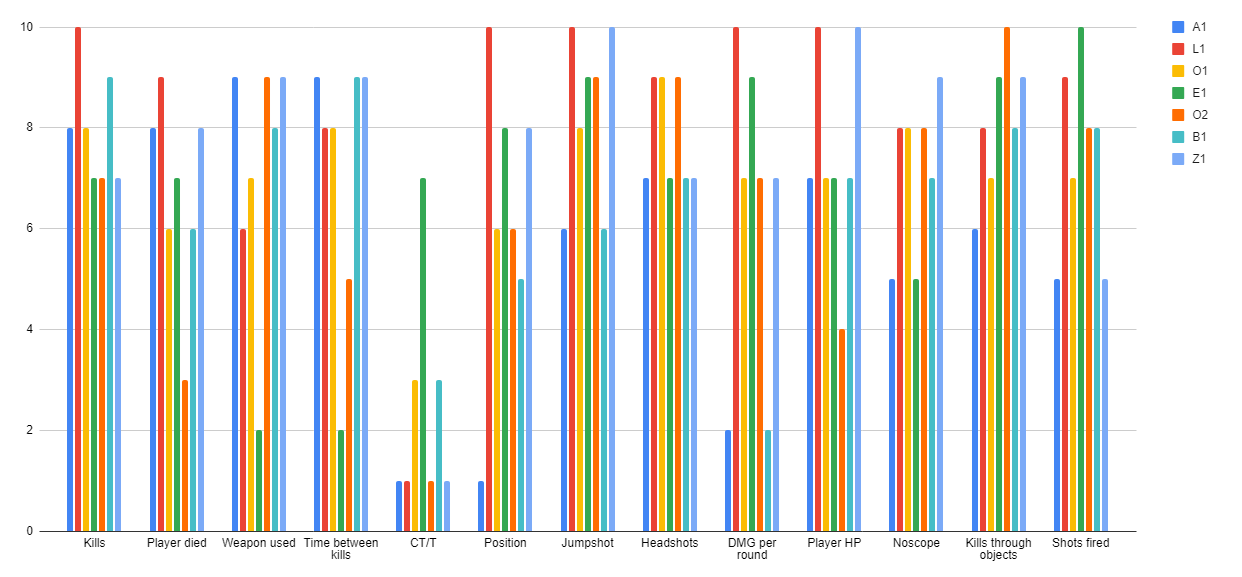
\includegraphics[width=17cm]{Images/All_results.png}
        \caption{Results from metrics rating}
        \label{fig:Barchart}
    \end{figure}
    \begin{figure}[H]
        \centering
        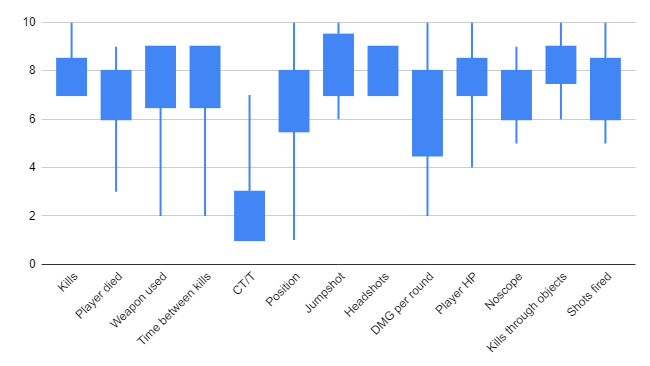
\includegraphics[width=17cm]{Images/boxplot.png}
        \caption{Box plot metrics}
        \label{fig:BoxplotMetrics}
    \end{figure}
    \begin{figure}[H]
        \centering
        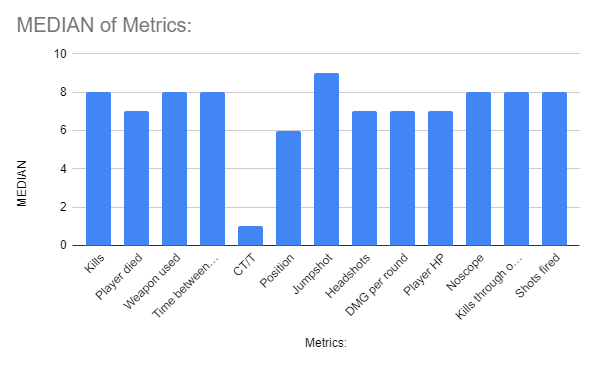
\includegraphics[width=17cm]{Images/medianMetrics.png}
        \caption{Median of metrics}
        \label{fig:medianMetrics}
    \end{figure}
    \textbf{Are there any metrics we forgot?}
    \begin{itemize}
        \item "After all, it is to create a metric to start running highlights when enemies are close to each other. Like in smokes or distance wise. Because if you are very close to each other on a site or something, highlights are rarely created there." (Participant L1, personal communication, April 10, 2024)
        \item "Well, hit percentage of the amount of bullets fired, right? I'm thinking, well, more or less. Oh, one second. Yeah, no, that's about it. The hit ratios are important to me. And maybe crosshair placement." (Participant B1, personal communication, April 21, 2024)
        \item "Kind of like Olofboost there." (Participant J1, personal communication, April 26, 2024)
        \item "Something you didn't mention was this movement thing." (Participant A1, personal communication, April 09, 2024)
        \item "Real movement players." (Participant O1, personal communication, April 30, 2024)
    \end{itemize}
\paragraph{Do you use any tool to create highlights?}
\begin{itemize}
    \item "I don't use anything. If I were to do it, I would use something that was simple and fast. Which fixed nice highlights. Which I could save and display. So, share those that might be able to be sent on discord directly. Or similar. Like GIFS." (Participant L1, personal communication, April 10, 2024)
    \item  "Yeah, FaceIt, like the FaceIt one." (Participant B1, personal communication, April 21, 2024)
    \item "And I use medal just to do it manually."(Participant B1, personal communication, April 21, 2024)
    \item "No, no more than the automatic that comes, for example, on e-sportal or results or something like that." (Participant J1, personal communication, April 26, 2024)
    \item "And then there's also GeForce Experience as well." (Participant J1, personal communication, April 26, 2024)
    \item "I used Medal around a year and a half ago. Then there was a lot of recording" {aiimar}
    \item "Leetify" (Participant O1, personal communication, April 30, 2024)
    \item "Yeah, Gif your game. Gif your game, but that's all." (Participant O2, personal communication, April 16, 2024)
    
\end{itemize}

\section{How do the perception of what makes a good highlight differ between novice and experienced players}
In the interviews, the biggest difference between novice and experienced players was in the specificity of the answers, those with less experience had a harder time explaining what they liked in a highlight. There was also less real life examples of highlights from those who had less experience.



\chapter{Discussion GIVE TAUGHT}
\label{chp:discussion}
\section{On the content}
\section{Discussion interviews}
The interviews were focusing on the metrics and what people liked about highlights. It lays a baseline on what metrics should be included and what metrics we already have included should be valued. The individuals we interviewed had different experience with highlights, Counter Strike 2 and other FPS games. Out of the 8 interviews we conducted, all had at least played one game of Counter Strike and knew of the game. Some with more experience than others. Many of the interviewees had a lot of experience with the Counter Strike scene and are or have been invested in the game for years, while others have just a couple of games under their belt.\\\\
The first question we asked the interviewees was, "What is your experience with Counter Strike or other FPS games?". From this question, we can have a broader aspect of what people with different experience think of such a topic as highlights in a game such as Counter Strike. The result we got from the question was that 6 out of 8 had a lot of experience in the game Counter Strike. While one interviewee had minimal experience with the game and another did not have much experience in Counter Strike but in other FPS games. One interviewee said, "I've been playing CS since I was a kid, more or less, 1.6. And then Source and all that. And then I started playing CS a lot in 2014. And have been playing CS since then every week. Since 2014 approximately. With some breaks here and there. But relatively regularly every year I played CS."\\\\
The second question we asked was "What is your experience with highlights in FPS games?". The result we got from this question was that most of the interviewees knew what they were, or with reference to other activities could understand the concept of a highlight. Many of the interviewees that had a lot of hours in Counter Strike had used programs such as Medal or similar to record the last 30 seconds or more to later edit or just save the clips. Others also answered with automatic clipping tools from sites such as Leetify and Esportal. Two out of the eight interviewees had no experience with highlights in FPS games.\\\\
The third question we asked, "What do you think is the most memorable highlight in Counter Strike history?". Here again the interviewees with a lot of hours in Counter Strike could reference highlights from the e-sport scene. Highlights that were mentioned was "happy 1Deag ace on Banana" (Participant B1, personal communication, April 21, 2024) which happened during the game between the e-sport teams "EnVyUs vs TSM" where the player Happy eliminates the whole enemy team with the weapon Desert Eagle during DreamHack Open London 2015. Another interviewee mentions, "After all, I have both famous ones from big tournaments or matches like Coldzera when he jumps and shoots on Mirage." 
(Participant L1, personal communication, April 10, 2024) which refences to a match between "Luminosity vs Liquid" during MLG Columbus 2016. The last refrence we get to e-sport matches is with an interviwee that says, "What I think is the best? Off the cuff, what pops into my head is Hiko. When he was clutching Dust 2 or something like that." Which references to the clip of the pro player Hiko getting a 180 degree flickshot on an enemy hiding behind a door on the map Dust2 during EMS One Katowice 2014 major.\\\\ 
What we can take away from this is that experienced players could give more concrete examples of highlights, but those with less knowledge could still give a vague answer of scenarios where a highlight would be applicable. 
The other interviewees answered with more general answers such as highlights that they had experience on their own, such as when they eliminated four players in a single round or when they eliminated the whole enemy team.\\\\
The follow-up question to the previous question is "What makes the highlight memorable?". Here we get interviewees referencing to casters of e-sports games "For me, that's what makes a good highlight. Precisely the part that lifts it is the skill demonstration. But also when the commentator is so damn hyped. That combination to me is absolutely fantastic. You get a lot of everything. If it's not from the clip, it's from the commentator. This for me means a lot. If it is no commentator. Which it is not when you play yourself. Then music can be the supporting part. That you have music that is timed with the shot or similar." (Participant A1, personal communication, April 09, 2024) another answered "The casters. Caster. Yeah. I suppose also the importance of the round". Others mentions the technical skills of the player, they won an impossible round or one answered "It must be something cool that happened. The more kills, the better. The faster the kills, the closer the kills are to each other, the better. The more shady the weapon, if you do something cool with it, the better." (Participant O1, personal communication, April 30, 2024). An important thing to notice from these answers are that many mentioned casters as an important part of highlights, especially in the e-sport scene. This is a valid input, but not in the scope of our proof of concept.\\\\
The fourth questions we asked was "What makes a good highlight?". From these questions we got a lot of different answers. One interviewee answered with "Quick succession. Quick responses. Like going from one to the other in rapid succession. And quantity of kills, usually." (Participant B1, personal communication, April 21, 2024) while another answered with "I have a hard time pointing to a thing. But if I have to point to one thing, it's one taps. I think that is absolutely fantastic. I think that is always worth including in a highlight. Deagle OneTaps. It could be AKs. If you do it several times in the same round, or you have 5 kills via OneTaps." (Participant A1, personal communication, April 09, 2024). These answers focus on the technical skill aspects of the highlights, while one interviewee said "A good highlight is made when there are a lot of people watching at the same time, when a good commentator at a professional match does a lot. And the circumstances, such as the thing that he is in Sweden and does such a thing against a non-Swedish team, means that everyone gets extra hyped."(Participant J1, personal communication, April 26, 2024) about the pro-scene and on individual level said "Then it is probably important that you want to play with friends. So that they actually see you. And the best thing is if it's one against five or similar so that everyone can see you when you play." (Participant J1, personal communication, April 26, 2024) focusing more on the social aspect of highlights and that it is something that gets the crowd or friends going. So from this we can gather that depending on the context of the game context and what scene players are playing in, there is a difference on what is considered highlight worthy.\\\\
Question five was about valuing metrics we provided to the interviewees from 1 to 10. Interesting takes from the average is that the team side has very low impact on a highlight.\\\\
Question six was, "is there any metric that we have forgotten?". On this question, one interviewee answered, "Something you didn't mention was this movement thing." which we did not include in the metrics but could be worth thinking about when developing the algorithm. One problem with accounting for movement is that it is hard to do, and what should be considered when looking at movement. Such, if a player moves fast between kills or if a player b-hops cross the map and eliminates an enemy. Another interviewee said, "The hit ratios are important to me. And maybe crosshair placement." Shots fired could be swapped out to hit ratio because as there could be situation where more bullets are necessary such as shooting through walls or where there is damage fall-off based on distance. Crosshair placement is also hard to weigh because of the implementation technicality, but it could be implemented. One interviewee said, "After all, it is to create a metric to start running highlights when enemies are close to each other. Type in smokes or distance wise. Because if you are very close to each other on a site or something, highlights are rarely created there. That they passed each other, were close to each other or that they did not see each other. Something along those lines.". To measure times when allies and enemies are in proximity to each other in a smoke or similar will also be hard to implement because of the technicality of the metric, but it could also be done. \\\\
Question seven "Do you use any tool to create highlights?" most interviewees answered that they had either used tools such as Medal, Faceit's highlight clipper, Esportal's highlight clipper. One interviewee answered, "I don't use anything. If I were to do it, I would use something that was simple and fast. Which fixed nice highlights. Which I could save and display. So, share those that might be able to be sent on discord directly. Or similar. like GIFS". So simplicity and portability would be important.\\\\
The follow-up to the question above was "What do you do with the highlights?". Where some interviewees answered that they put them on YouTube in compilations with other clips, and some share them with friends. So highlights is mostly used to recap good moments and to be able to share them with friends and others.\\\\
Based on the answers we got from the questions, we now have a baseline of what we should value the different metrics. We also got new thoughts on what people look for in highlights and got examples of highlights that the interviewees liked. During the interviews, we also noticed a stark difference in the specificity of answers with the people who had more experience with Counter Strike than those without. 
\section{Discussion on the algorithm and survey}
As we tried to make an algorithm that outputted better highlights, based on the results we got from the survey, our algorithm managed to get the slight edge as it was preferred 6 out of 9 times. As Allstars algorithm is not public, it is not possible to explain what metrics are focused on and hard to do a full on comparison against our algorithm. The information we get is the outputted round by Allstars. To understand why our video clips were preferred, we need to look at the difference between the videos and the answers the respondents gave. The matches where there was a major preference to one of the videos was the matches 2, 3, 5, 7, 8 and 9. Worth mentioning is that out of 19 matches, 9 times Allstar and our algorithm outputted the same round. This seems to happen when a player only gets one round with 4+ kills and the rest are 1 and 2 kills. This could simply be that the player had one very good round and the remaining rounds were poorly played. This could mean the more similar rounds, the more difference in what our algorithm will pick and what Allstar will pick. 
\subsection{Match 2}
In match 2 both clip A and B included 2 kills, but the winning clip B included a kill with the knife which was liked by the respondents. There were also comments on that clip A was messy. It is however important to remember that our algorithm does not account for things such as movement or crosshair placement, which could be considered messy. We do not know if this is something that Allstar takes into account.
\subsection{Match 3}
In match 3 we have the clips, A with 4 kills and B with 3 kills. Key difference in clip B the player did not die in the end of the clip which our algorithm takes into account. Even though in clip A which is from Allstar had 4 kills, the majority picked clip B with only 3 kills. One response that preferred our video B was "In video A the player dies, I do not thing that is a good end of a highlight" So here our check for if the player died mattered. Another respondent answered with "Video A was a nice 4K with a 2 kill spraydown. Video B was more average" and seemed to value the 4th kill and a multikill highly, which gets lowered in our algorithm because of the death in the end of the clip. A discussion could also be held again for movement as one player wrote "Better checks on corners and utilized utilities and safe playmaking" as we do not check for that in our algorithm, but our clip was still chosen.
\subsection{Match 5}
In match 5 clip A contains 2 kills and clip B contains 3 kills. In this match the player dies in clip A and not in clip B which two respondents answered with "In video B he does not die, and gets most of the kills" and "He didn't die, and won round". Even though there might need to be more data collected, the effect of dying seems to be important to players and our algorithm takes this into account. 
\subsection{Match 7}
In match 7, clip A contains 2 kills and 1 team kill and clip B contains 2 kills. The player does not die in any of the clips. The majority prefers clip B which was from our algorithm. The respondent's reasoning for this was a bit of spread, as one said "More kills, as well as a nice 2K spraydown. First shot was especially clean" and "I bet your algorithm is counting team kills as normal kills" even though the last kill was team kill they still picked clip A. Our algorithm does not count team kills as kills. The only respondent that picked clip B and had a reasoning said "Just a better round, he knows what he is doing and plays around the enemies making mistakes". There could be a case for the succession of kills in clip B was faster than in clip A but no comments about this were made.
\subsection{Match 8}
Match 8 had two highlights. Highlight A contained a nice clutch with 3 kills, and highlight B had a good glock round with two kills. Here highlight A won because of the clutch, and it had more and cleaner kills. The amount of kills is something that Allstar at least counts, and we can assume that is taken into account, since the title of their clips have the amount of kills in them, as well as the weapon that was used. Since clean came up a few times, this might relate to the accuracy, and that does our algorithm consider. In highlight B the opponent missed a few of his shots, only showcasing that the player should have died, but only survived to clutch the round because of the bad play by his opponent.
\subsection{Match 9}
In match 9, highlight B includes three quick kills in the beginning, with a nice clutch at the end, showing off the gamesense of the player, tricking the player that he had gone back to a different site, while in highlight A, there are three nice kills, two that are trough a smoke. Here the respondents said that they liked highlight B better, since it was more tactical, and the glock kills were nice. The two fast glock kills is something that our algorithm takes into account, but in this case, highlight B was not chosen by our algorithm, and instead chosen by Allstar. We can not know if this is something that they are taking into account, but our algorithm takes both weapon and time between kills into account. Here the AK47 kills got chosen since they are a more difficult weapon. Both highlights are fast paced, and as we can see but the weapons weights might need to be adjusted to make a highlight like this be chosen by our algorithm. Currently, the weapons might be slightly too much of a factor. 







% All references are in a separate file: thesis-refs.bib
\bibliography{thesis-refs}
\bibliographystyle{IEEEtranS}


\appendix
\chapter{Supplemental Information}


% DO NOT CHANGE BELOW
% This part makes sure that the last page is even with BTH-logo.
% -------------------
\cleardoublepage
\thispagestyle{empty}
\vspace*{\fill}
\clearpage{\thispagestyle{empty}}
\changepage{3cm}{1cm}{-0.5cm}{-0.5cm}{}{-1.5cm}{}{}{}
\vspace*{\fill}
\center

{\bthcsnotextlogo{3cm}}
\\
\noindent\makebox[\linewidth]{\rule{\textwidth}{1pt}} 
Faculty of \faculty, Blekinge Institute of Technology, 371 79 Karlskrona, Sweden
% -------------------

\end{document}
